\documentclass{ieeeaccess}
\usepackage{cite}
\usepackage{amsmath,amssymb,amsfonts}
\usepackage{algorithmic}
\usepackage{hyperref}
\usepackage{multirow}
\usepackage[table]{xcolor}
\hypersetup{colorlinks = true, allcolors = accessblue}
\usepackage{caption}
\DeclareCaptionFont{ieeeblue}{\color{accessblue}}
\DeclareCaptionLabelFormat{myformat}{\figcapfont{\textbf{#1}\textbf{#2}}}
\captionsetup{labelfont={bf,ieeeblue},labelformat=myformat}

\usepackage{graphicx}
\usepackage{textcomp}
\def\BibTeX{{\rm B\kern-.05em{\sc i\kern-.025em b}\kern-.08em
    T\kern-.1667em\lower.7ex\hbox{E}\kern-.125emX}}


\begin{document}
\history{Received July 24, 2020, accepted August 4, 2020, date of publication August 10, 2020, date of current version August 20, 2020.}
\doi{10.1109/ACCESS.2020.3015227}

\title{Open Set Audio Recognition for Multi-class Classification with Rejection }

\author{\uppercase{Hitham Jleed}\authorrefmark{\href{https://orcid.org/0000-0002-1714-5578}{
\includegraphics{img/orcid.png}} 1,2}, \IEEEmembership{Student Member, IEEE}, and
\uppercase{Martin Bouchard \authorrefmark{\href{https://orcid.org/0000-0002-1165-438X}{
\includegraphics{img/orcid.png}} 1}},
\IEEEmembership{Senior Member, IEEE}}
\address[1]{School of Electrical Engineering and Computer Science, University of Ottawa, Ottawa, ON K1N 6N5, Canada}
\address[2]{Department of Electrical and Computer Engineering, Elmergib University, Alkhoms, Libya}

\tfootnote{This work was supported in part by a Natural Sciences and Engineering Research Council of Canada (NSERC) Discovery grant and by the Libyan North American Scholarship Program (LNASP) scholarship fund. }

\markboth
{H.Jleed \headeretal: Open Set Audio Recognition for Multi-class Classification with Rejection}
{H.Jleed \headeretal: Open Set Audio Recognition for Multi-class Classification with Rejection}



\corresp{Corresponding author: Hitham Jleed (e-mail: hjlee103@uottawa.ca).}


%============================================================================= Start FROM HERE ===========================
%%%%% abstract
\begin{abstract}
Most supervised audio recognition systems developed to this point have used a testing set which includes the same categories as the training set database. Such systems are called closed-set recognition (CSR). However, audio recognition in real applications can be more complicated, where the datasets can be dynamic, and novel categories can ceaselessly be detected. Hence, in practice, the usual methods will assign to these novel classes labels which are often incorrect. This work aims to investigate audio open-set recognition (OSR) suitable for multi-classes classification recognition, with a rejection option for classes never seen by the system. A probabilistic calibration of a support vector machine classifier is utilized and formulated under the open-set scenario. For this, it is proposed to apply a threshold technique called peak side ratio (PSR) to the  audio recognition task. A candidate label is first examined by a Platt-calibrated support vector machine (SVM) to produce posterior probabilities. The PSR is then used to characterize the distribution of posterior probabilities values. This process helps to determine a threshold in order to reject or accept a particular class. Our proposed method is evaluated on different variations of open sets, using well-known metrics. Experimental results reveal that our proposed method outperforms previous OSR approaches over a wide range of openness values.
\end{abstract}

\begin{keywords}
Open-set recognition, audio recognition, sound event recognition, multi-class classification, support vector machine, peak side ratio.
\end{keywords}

\titlepgskip=-15pt

\maketitle
\setcounter{page}{146523}
\section{Introduction}
\label{sec:introduction}
Closed-set recognition systems (CSR) are often governed by misleading assumptions, where all testing and training data are taken from the same database, often with equal distribution. Under these assumptions, several algorithms have achieved significant success in many applications of machine learning. Machine learning algorithms are able to perform empirical risk minimization very well, using their ability to handle large feature spaces and to identify outliers. However, these assumptions do not reflect some practical applications in which out-of-set data may be encountered. When data from a new class occurs, it is classified as one of the known classes. Even if this sample lies far from any of the training samples, it may be classified with a high probability, that is, the algorithm will not only be wrong, but it may also
\\

% environment
\begin{footnotesize}
The associate editor coordinating the review of this manuscript and approving it for publication was Ioannis Schizas \href{https://orcid.org/0000-0002-1714-5578}{
\includegraphics{img/orcid.png}}.

\end{footnotesize}

\noindent be very confident in its results  \cite{1}. A more practical problem is open set recognition (OSR), where samples of classes not seen during training may show at testing time. OSR systems need to formulate new assumptions that can balance both empirical risks: the risk of a tested sample misclassification and the risk of labeling unknown space \cite{2}. Any signal or event in an open-set classification scenario will be under one of the following categories  \cite{3}:
\begin{enumerate}
	\item Known classes (KCs): the classes for which data samples are labeled positive for training and testing.
	\item Known unknown classes (KUCs): Classes that are seen at training time, but at validation time they are considered as unknown, to build unknown models. These are used for tuning parameters.  
	\item Unknown unknown classes (UUCs): Classes that have not been seen in the training or the validation stages. They appear only in the testing stage.
\end{enumerate} 

In this paper, we aim to solve the open-set audio or sound event identification and detection problem by setting a threshold to detect new instances and new classes, based on the peak side ratio (PSR) of calibrated posterior probabilities, rather than applying a threshold on the probabilities themselves. \\
Experiments need to be carefully designed for evaluating multi-class open set recognition. We use well-known data sets retrieved from the Detection and Classification of Acoustic Scenes and Events (DCASE) challenge  \cite{4}. Because open-set recognition requires an experimental system that uses classes unseen during training, we take some classes from the database to simulate the unknown classes. A one-vs-rest multi-class method is used to implement the radial basis function support vector machine (RBF SVM). The system has as many classifiers as the number of known classes. During the test phase, the classifiers predict the posterior probability of each class for the tested sample. The posterior probability under a closed set setting can easily predict the tested sample’s distance from the separating hyperplane, and the highest probability value leads to the class to which it belongs.  
However, the system in an open-set setting does not know the unknown classes and thus cannot estimate the probability of unknown classes. Instead, we compare the distribution of posterior probabilities of all classes for the tested sample. If the highest probability value is far away from other values, this class is considered as known and is recognized. Otherwise, it will be considered as an unknown class. We propose the PSR to measure this aspect. This measure was introduced in  \cite{5}[5] for face recognition purposes. In this work, we propose to include the PSR in audio recognition tasks and to validate its use. Consequently, our proposed algorithm consists of: deriving a set of calibrated posterior probabilities values; deriving a PSR for the tested samples using the set of probabilities values; comparing the PSR to a rejection threshold; and rejecting the unknown samples if the rejection threshold is less than or equal to the PSR. 

The structure of this paper is as follows. In section \ref{sec:II},we present the literature review; 
in section \ref{sec:III}, we clarify some definitions and notation concepts of open-set scenarios; 
in Section \ref{sec:IV}, we describe feature extraction; 
in Section \ref{sec:V}, we illustrate the evaluation metrics used to measure the system performance;
in Section \ref{sec:VI}, we propose our method of classification; 
and in Section \ref{sec:VII}, we evaluate the performance of our proposed method and compare it with other methods.
A conclusion then follows in Section \ref{sec:VIII}.


\section{LITERATURE REVIEW} \label{sec:II}
In this section, we review recent work in the literature which explicitly deals with audio features representations \ref{subsec:features}, audio recognition \ref{subsec:recog} and open-set scenarios \ref{subsec:openscen}. 

\subsection{Audio-Features Representations} \label{subsec:features}
Feature extraction is a critical step in audio/sound event classification. An efficient representation must capture the most significant sound properties for the task. Several efforts have been made to harvest data with respect to dimension and sample size. The most common features used in audio recognition are the Mel-frequency Cepstral Coefficients (MFCCs). In the speech processing domain, the first thirteen MFCC values have been verified to be particularly pertinent due to their approximate separation of the glottal excitation from the vocal tract \cite{6}. The MFCCs are perceptual features computed from the short-term Fourier transform. The power spectrum bins are computed and scaled with Mel-frequency scaling. The output is then framed into a number of filter banks, corresponding to overlapping triangular filters. Finally, a discrete cosine transform (DCT) is applied to the filter bank magnitude logarithm outputs, producing vectors of nearly decorrelated MFCC features. By equally spacing the frequency bands on the Mel-scale, the MFCC decomposition resembles how sound is perceived by humans, and provides statistics of how the frequency content changes in different spectrum bands, which make them useful for audio recognition. Other features have been used for audio classification, including but not limited to: MPEG-7 audio features \cite{7},feature representation based on bag-of-audio-words \cite{8}, and indexing-based features \cite{9}. Also, features based on the discrete Hartley transform \cite{10} have been shown to be useful in audio scene classification applications. \\
Although the choice of features affects the overall classification performance, this choice is not key to the main objective of this paper, which is to investigate the benefit provided by the PSR measurement for open-set problems in audio classification. This paper uses the MFCC features as the base features because of their widespread use and since they have proven to be effective in recognizing the structure of acoustic/speech/audio signals (sometimes in combination with other features, as we do in this paper). 

\subsection{Audio detection/recognition} \label{subsec:recog}
Many of the classification methods that can be encountered in the literature detect presence/absence of a specific event during a period of time. Several organized challenges have been created for acoustic events detection and recognition to evaluate these research methods. These challenges regularly report progress and provide useful resources for research, such as the SiSEC evaluation for signal separation \cite{11}, the CHiME speech separation and recognition challenge \cite{12}, the MIREX competition for music information retrieval \cite{13}, and the DCASE 2013-2019 challenges \cite{4}.\\
Other notable previous work includes \cite{14}, where Lopatika et al. used an SVM classifier to discern between classes of hazardous situations. They used long-range audio features to classify four predefined classes and then localize them. Similarly, Hilal et al. \cite{15} used linear discriminate analysis (LDA) and SVM classifiers to identify and localize a set of predefined environmental sound events.


\subsection{Open-set Scenario} \label{subsec:openscen} 
In the audio domain, there have been few previous publications investigating open-set scenarios. Battaglino et al. \cite{16} applied the open-set method to audio scene classification, where a specific type of 1-class SVM has shown promising results for open-set recognition. Recently, Krstulovic \cite{17} published a book chapter illustrating the importance of the open-set problem in the audio domain and investigating the restrictions of the existing evaluation practices, such as using F1-score, precision, and recall. \\
The problem of road surveillance was considered in \cite{8}, where two hazardous situations were detected: car crashes and tire skidding. The bag-of-words dictionary technique was used to compute the occurrences of low-level features and assemble a high-level vector that has an equal dimensionality to the number of possible words in the dictionary. Crocco et al. \cite{18} made a good survey on audio surveillance methods, which dealt with a small group of sound classes. They also emphasized the challenges that a surveillance scenario faces.\\
The concept of open-set recognition has so far received more attention in image/face recognition tasks. Recent methods to detect unrelated samples in open-sets problems have been investigated by Scheirer et al. \cite{2}, where a one-vs-all setting was used to formulate the problem of open set image recognition.  The open space risk and the empirical error were aimed to be balanced. The work was then extended in \cite{3} by introducing the 1-vs-set machine with the compact abating probability model. Jain et al. \cite{19} introduced the Weibull-calibrated multi-class SVM classifier for open-set image recognition. They showed promising results based on minimizing open space risk, which is a compromise between computing capabilities and support vector estimations. Bendale et al. [20] proposed a Nearest Non-Outlier (NNO) algorithm and gave the definition of open word image recognition, where the unknown samples are not a static set. They extended their work in \cite{21} by modifying a deep learning structure for open-set recognition, combined with the concept of the penultimate layer with meta-recognition \cite{22}. Similarly, in radar image recognition, Roos and Shaw \cite{23} used open-set recognition on high range resolution radar and formulated an automatic target recognition. \\
Our proposed solution to distinguish known and unknown events is related to estimating the posterior probability. The recognition algorithm is implemented according to the SVM classifier framework. The SVM has a good reputation as a robust classifier due to the optimal margin gap between separating hyperplanes. The decision function in a Platt-calibrated SVM provides the posterior probability of each classifier. Since we deal with multi-class recognition, the decision functions are combined in a one-vs-rest fashion. 
However, a traditional SVM works for the closed-set problem, where the testing set includes the same categories as the training set database. The open-set recognition cannot simply use the maximum posterior probability (MAP) estimate over the known classes as the best solution, because the probability estimation of unknown classes is not possible. In addition, the probability estimation does not provide a sufficient scale when novel class data are far from any training data. The PSR measurement is proposed for audio classification in our work to make a rejection decision by defining the relationship between the maximum posterior probability value and other values. If the PSR is bigger than a certain threshold, the sample is rejected and labeled as an unknown class. A large PSR value means that the recognition is questionable due to ambiguity and yields rejection. The threshold is computed a priori during a validation step, where the system is inspected under a variety of thresholds. The best threshold found is then considered predefined and constant during the real experiments.\\
As can be seen from the literature, most of the previous works on open-set scenarios have been done in image processing applications. Therefore, in this paper we investigate the applicability of some techniques previously developed for image classification and evaluate their use and performance in the context of audio classification, where the signals have different characteristics.
 




\section{NOTATION AND DEFINITION} \label{sec:III}
Let us first establish preliminaries related to open-set recognition. The openness of a given problem is an estimate of the need for rejection in order for a proper solution to be found. It measures the potential for the existence of sound classes that are not fully known in the training and validation stages. Therefore, some classes are withheld as unknown to simulate this scenario. Let $Y$ be the set containing all class labels in a given data. Scheirer et al. \cite{b2} defined three quantities: target, known, and unknown. We call $Y$ the set containing all the class labels in the given dataset and use the subscripts $t$,$k$, and $u$  for the target, known and unknown sets, as described by the Venn diagram in fig. \ref{fig:fig1}.
\begin{figure}[t!]
	\centering
	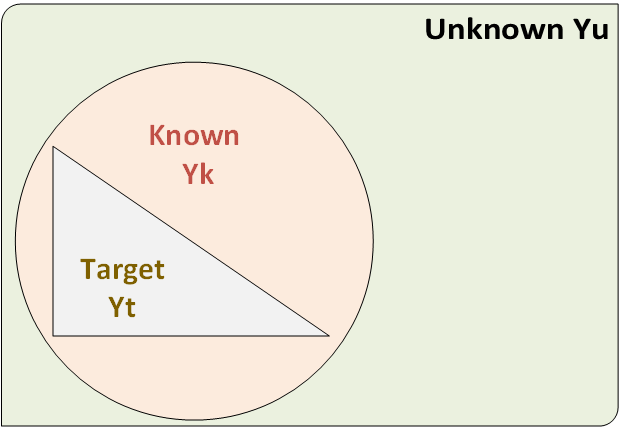
\includegraphics[width=0.45\textwidth]{img/venndiagram.png}
	\caption{Venn diagram of acoustic classes. $Y_{t}$    is the set of known target classes to be recognized,   $Y_{k}$ is the set of all known classes used in training, $Y_{t},Y_{k}$ and $Y_{u}$  is the set of classes used during testing. $Y_{train}=Y_{t} \cup  Y_{k}  $  and $Y_{test}=Y_{t} \cup  Y_{k} \cup  Y_{u} $ }
	\label{fig:fig1}
\end{figure}
The data from the target and known negative classes are used for training  $Y_{train}=Y_{t} \cup  Y_{k}  $ ,  , and representative data from known classes are used only to evaluate open-set classification. The testing dataset is a combination of all classes  $Y_{test}=Y_{t} \cup  Y_{k} \cup  Y_{u} $ . The openness is defined in \cite{b1} as: 

\begin{equation}
Openness=1-\sqrt{\frac{2\times \left | Y_{t} \right |}{\left |Y_{k}\right |+\left |Y_{u}\right |}}.
\label{eq1}
\end{equation}
where $ \left |. \right |$  here represents the number of elements in each set. The openness ranges from 0 to 1, where 0 represents a completely closed-set problem. Increasing the number of classes available in the training phase leads to a decrease in openness. The square root slows down the openness from quickly moving toward the 1 value. If we define the sets of training and testing classes as  $ Y_{train} \subset Y$ and $ Y_{test}\subset Y $ , the novel classes will be  $ Y_{u}=\left \{ y|y\in Y_{test} \textrm{ and } y \notin Y_{train} \right \} $.

\section{FEATURES EXTRACTION}  \label{sec:IV}
In contrast to video signals, an audio signal has quick variations within a short time. Hence,  the input audio stream is first framed into groups of P overlapping segments. Each segment has a duration of N samples and is multiplied by a Hamming window. The choice of the segment duration is a trade-off. If the length is too short, it may be unable to represent accurately fine details of the low-frequency components (from poor frequency resolution). Conversely, if it is too long, the frame cannot describe the short-time changes in the audio signal. We used N  =2048 samples and 512 samples for the segment shift. Before executing any training or classification, the sounds under investigation need to be characterized and represented in a form that can easily be computed. Feature extraction is the process of extracting useful discriminative information from the raw waveform signals and producing a compact set of feature vectors.

\subsection{Mel frequency Cepstral Coefficients}
As previously mentioned, extracting MFCCs is a widely used procedure in speech classification applications. The frequency bands are equally spaced on the Mel-scale to resemble how humans perceive sound. For speech or speaker recognition, 13 MFCCs are enough to encode information about the vocal tract \cite{24}. However, there is no optimal number of MFCCs to be used for a non-speech application. In this work, we adopt the choice made in the DCASE challenge of using 40 coefficients \cite{25}. The MFCC coefficients are computed using the following steps. The signal is first divided into frames. The frame  $x_{p}(n)$ with length N is pre-emphasized with a high-pass filter to compensate for a spectral slope. The transfer function is $ H(z)-1-\alpha Z^{-1} $. $0.9\leq\alpha\leq1.0$. We used $\alpha =0.97$. The spectral slope is the tendency of natural audio signals to have less energy at high frequencies. Each frame is multiplied with a Hamming window  $ w(n)=0.54-0.46\cos (\pi n/N) $, followed by a discrete Fourier transform. In practice, this is referred to as the (discretized) short-time Fourier transform (STFT)  \cite{26}: 
\begin{equation}
X_{p}(k)=\sum_{n=0}^{N-1}x_{p}(n)w(n)e^\frac{-j2\pi kn}{N}
\label{eq2}\end{equation}
with $k=0,1, … ,N-1$ coefficients and $p=0,1, … , P-1$ frames. $ X_{p}(k) $  corresponds to the content at the discrete frequency $ f(k)=kF_{s}/N $,where  $F_{s}$  is the sampling frequency. The result is a matrix of size $ N\times P$  The spectrum $ \left | X_{p}(k)\right | $ is then scaled in both magnitude and frequency. The frequency is logarithmically scaled as in (\ref{eq3}): 
\begin{equation}
{X}'_{p}(m)=\ln\left (\sum_{k=0}^{N-1}\left | X_{p}(k) \right | H(m,k)\right )
\label{eq3}
\end{equation}
with $m = 1, 2, … , F$ , where $F$ is the number of filter banks, and  $p = 0,1, … , P-1$. The filter bank output is computed by the product of the magnitude spectrum $ \left | X_{p}(k) \right |$ and the Mel filter bank $H(m,k) $ described by an  $F\times N$ matrix. The Mel filter bank $H(m,k)$ triangular responses are computed in terms of the center frequencies $f_{c}(m)$ as in (\ref{eq4}):


\begin{equation}
\resizebox{0.17\hsize}{!}{$H(m,k)=$}
\begin{cases}
0                                           &  \resizebox{0.25\hsize}{!}{$f(k)< f_{c}(m-1)$} \\ 
\frac{f(k)-f_{c}(m-1)}{f_{c}(m)-f_{c}(m-1)} &  \resizebox{0.4\hsize}{!}{$f_{c}(m-1) \leq f(k)< f_{c}(m)$}\\ 
\frac{f(k)-f_{c}(m+1)}{f_{c}(m)-f_{c}(m+1)} &  \resizebox{0.4\hsize}{!}{$f_{c}(m) \leq f(k)< f_{c}(m+1)$}\\ 
0                                           &  \resizebox{0.25\hsize}{!}{$f(k)\geq f_{c}(m+1)$} 
\end{cases}
\label{eq4}
\end{equation}
The filter bank center frequencies in Hz are obtained from uniformly distributed frequencies in the Mel scale. There are several formulae in the literature to convert a frequency in Hz to a frequency in Mel. We use the one found both in the Librosa Python library \cite{27} and the MATLAB Auditory Toolbox \cite{28}, given as:(\ref{eq5}):
\begin{equation}
f_{Mel}=2595.0 \times log\left ( 1+\frac{F_{HZ}}{700} \right )
\label{eq5}
\end{equation}
A uniform Mel scale frequency resolution is then calculated based on a logarithmic scaling of the frequencies, by
\begin{equation}
\Delta f_{Mel}=(max(f_{Mel})-min(f_{Mel}))/(F+1)
\label{eq6}
\end{equation}
The Mel scale center frequencies are computed by $ F_{c,Mel}(m)=m\Delta f_{Mel} $ for m = 1, 2 ... F, from which the center frequencies $f_{c}(m) $  in Hz can be obtained. Applying the DCT to  $ {X}'_{p}(m) $ provides the MFCC coefficients,
\begin{equation}
c_{p}(r)=\sqrt {\frac{2}{F}}\sum_{m=0}^{F-1} {X}'_{p}(m)cos(r\frac{\pi}{m}(m-\frac{1}{2}))
\label{eq7}
\end{equation}
where  $c_{p}(r)$  is the $r^{th}$ MFCC of the $p^{th}$ frame, and r = 0,1... 39. Features are then collected, including the coefficient for frequency zero. We also compute delta "differential coefficients" that can capture the dynamic properties of the cepstrum, calculated using the following formula:
\begin{equation}
d_{p}=\frac{\sum_{n=1}^{Nd}n(c_{p+n}-c_{p-n})}{2\sum_{n=1}^{Nd}n^{2}}
\label{eq8}
\end{equation}
where $d_{p}$  is a delta coefficient for frame p, and $N_{d}$  is the number of coefficients selected. We use $N_{d}=9$   in our proposed system.

\subsection{FREQUENCY-DOMAIN FEATURES}
While MFCCs are well-known features in speech classification applications that resemble how people interpret sound, for audio recognition additional features are often used, such as spectral sparsity, spectral flux, and spectral centroid used in this work.\\
Spectral sparsity is defined as a normalized maximum frequency, as the following:
\begin{equation}
Sparsity(p)=\frac{max\left \{ \left | X_{p}(1),...,X_{p}(N)) \right | \right \}}{\sum_{k=0}^{N-1}X_{p}(k)}
\label{eq9}
\end{equation}
The spectral flux captures the change of spectra between two successive segments. It is computed as in \cite{22} by taking the squared difference between two consecutive spectral contents:  
\begin{equation}
flux(p)=\sum_{k=0}^{N-1}(\left | X_{p}(k) \right |-\left | X_{p-1}(k) \right |)^{2}
\label{eq10}
\end{equation}
The spectral centroid computes the center of gravity of the spectrum. For each $p^{th}$ frame, it is computed as in (\ref{eq11}):
\begin{equation}
Centroid(p)=\frac{\sum_{k=0}^{N-1}(k+1)\left | X_{p}(k) \right |}{\sum_{k=0}^{N-1} X_{p}(k) }
\label{eq11}
\end{equation}

%======================== cut



\section{EVALUATION METRICS} \label{sec:V}
The choice of statistics to use for evaluation of classification performance needs to be addressed. Metrics used in audio detection and classification include accuracy, F-score, precision, acoustic event error rate (AEER), and error rate (ER). Let TP, TN, FP, and FN denote the true positive, true negative, false positive, and false negative counts, as explained in \cite{29}. 

\subsection{PRECISION AND RECALL}
Precision is the portion of positives classifications that are computed correctly (true), while recall is the ratio of the total positive samples which are correctly detected by positive classifications. These can be calculated in two ways, macro-averaging as in eq (\ref{eq12}) and micro-averaging as in eq (\ref{eq13})
\begin{equation}
\begin{matrix}
\resizebox{0.422\hsize}{!}{$P_{mac}=\frac{1}{Nk}\sum_{i=1}^{Nk}\frac{TP_{i}}{TP_{i}+FP_{i}} $}
&
\resizebox{0.422\hsize}{!}{$ R_{mac}=\frac{1}{Nk}\sum_{i=1}^{Nk}\frac{TP_{i}}{TP_{i}+FN_{i}} $}
\end{matrix}
\label{eq12}
\end{equation}

\begin{equation}
\begin{matrix}
\resizebox{0.38\hsize}{!}{$ P_{mic}=\frac{\sum_{i=1}^{Nk}TP_{i}}{\sum_{i=1}^{Nk}(TP_{i}+FP_{i})} $}
&   &
\resizebox{0.38\hsize}{!}{$R_{mic}=\frac{\sum_{i=1}^{Nk}TP_{i}}{\sum_{i=1}^{Nk}(TP_{i}+FN_{i})} $}
\end{matrix}
\label{eq13}
\end{equation}
In this work, we computed the average of precision and recall for all classes using macro and micro averages, treating all classes equally, as described in \cite{30}.

\subsection{AVERAGE ACCURACY AND F-MEASURE}
Following the definition of metrics as in \cite{31}, the average accuracy is computed as in (\ref{eq14})
\begin{equation}
A=\frac{1}{Nk}\sum_{i=1}^{Nk}\frac{TP_{i}+TN_{i}}{TP_{i}+TN_{i}+FP_{i}+FN_{i}}
\label{eq14}
\end{equation}
where the $i$ subscript refers to the $ i^{th} $ training class. The F-measure is a score that can represent both precision and recall in a single score. The general form of F-measure is computed as 

\begin{equation}
F-measure=\frac{(\beta^{2}+1)PR}{\beta^{2}P+R}
\label{eq15}
\end{equation}
where $ \beta $ is a parameter providing weights for both precision ($P$) and recall ($R$). We used $\beta=1$ in this work, as it is the definition of the F1-measure, a commonly used measure.

\subsection{CONFUSION MATRIX}
The accuracy metric provides an appropriate evaluation only if the class labels are uniformly distributed, which is the case of the closed-set recognition task also considered in this work. In this case, the confusion matrix $ CM(i,j) $ is a good technique to summarize the performance of multi-class classification. Each column of the matrix corresponds to an actual class, and each row corresponds to a predicted class. The diagonal of the confusion matrix shows the correct classification prediction $ i=j $ .In this work we used a row-wise normalized confusion matrix  $ CM_{n}(i,j) $ defined in \cite{32}, where each element is divided by the sum of elements in each row:
\begin{equation}
CM_{n}(i,j)=\frac{CM(i,j)}{\sum_{i}CM(i,n)}
\label{eq16}
\end{equation}

\subsection{REDUCED CONFUSION MATRIX}
The reduced confusion matrix is the confusion matrix reduced to a $ 2\times2 $ matrix to evaluate the open set performance \cite{23}. The classes of the matrix are the known targets and unknown targets, as shown in Table \ref{tab:table1}. The performance of the classifier can be computed based on how well these two classes are distinguished.  
\begin{table}[h]
	\caption{Reduced Open-set Confusion Matrix}
	\centering
\begin{tabular}{m{1.5em} m{5em} m{5em} m{5em}}
 	& \multicolumn{3}{c}{Predicted}\\
 	\parbox[t]{2mm}{\multirow{3}{*}{\rotatebox[origin=c]{90}{Actual}}} & 
 	& \cellcolor{lightgray} Known& \cellcolor{gray} Unknown\\ 
 	& \cellcolor{lightgray} Known &TP& \cellcolor{lightgray} FN\\ 
 	& \cellcolor{gray} Unknown & \cellcolor{lightgray} FP&TN\\ 
\end{tabular}
\label{tab:table1}
\end{table}

\subsection{ACOUSTIC EVENT ERROR RATE}
 This metric defined in \cite{33} is used to measure the classification errors in terms of substitutions  ($ S $), insertions ($ I $), and deletions ($ D $). Substitutions ($ S $)are the number of reference events for which an incorrect event was detected by the classifier. The remaining events are insertions ($ I $),defined as the number of classifier detections with no corresponding event, and deletions ($ D $)defined as the number of reference events with no corresponding classifier detection:
\begin{equation}
	\begin{matrix}
		S= min (FN,FP)\\
		D=max(0,FN-FP)\\
		I = max(0,FP-FN)
	\end{matrix}
	\label{eq17}
\end{equation} 
Given $ T $ as the number of detected events, the Acoustic Event Error Rate ($AEER$) is computed as in (\ref{eq18}),
\begin{equation}
	AEER=\frac{D+I+S}{I}\times 100
	\label{eq18}
\end{equation} 

\section{METHODOLOGY} \label{sec:VII}
Compared with closed-set audio classification, which has been investigated for decades, open-set audio recognition classification needs a special setup, methodology, and experiments, which can distinguish audio events of interest from frequent daily events. This section will discuss the proposed method in details.
\subsection{DATABASE}
We validate our proposed framework in an open-set audio recognition experiment by using a dataset that contains audio events recorded in an office-like environment retrieved from DCASE 2013  \cite{34} and from the Freesound online database \cite{35}. The recorded events have different sizes and varying noise levels. The sound event classes used are: short alert, clearing throat, cough, door slam, drawer, keyboard clicks, keys put on the table, knocking on door, laughter, mouse click, page turning, pen or pencil touching a table surface, phone, printer, speech, and switch. This is a challenging set to work with, as some of these sounds can be similar. To address open-set recognition, we randomly select six classes to build our models and keep the remaining ten classes as unknown classes. To create different levels of openness, for each setting 2\textendash5 classes from the known classes are considered as target classes. From the unknown classes, in each setting 3\textendash9 classes are selected. Experiments in multiple settings are performed, for a total of 28 combinations.

\subsection{SIGNALS PROCESSING}
The input audio files are preprocessed with normalization, frame segmentation and windowing. The sampling frequency is fixed for each file as 44100 samples/sec. Files that have different sampling frequencies are resampled to this value. Each audio file is normalized to maximum unit amplitude, to bring the gain of the entire track to its maximum without clipping. Due to the presence of silence frames and to avoid ambiguity in sound event labels, the system uses a Voice Activity Detection (VAD) technique to select the most energetic frames of the audio and to discard the rest. We divided each recording into frames with a small length of 20 ms, and $ 50\% $ overlapping. The actual $ ES_{pq} $ energies are computed in the frequency domain frame by frame, where $ p $ represents the frame index and $ q $ is a frequency bin. The noise energies $ En_{pg} $ are estimated independently for each frame. The first frame is considered a pure noise, and the algorithm adapts with each frame based on the moving average function $E{n_{pq}} = 0.94 \times E{n_{pq}} + (1 - 0.94) \times E{S_{pq}}$ This function is computed only when the signal energy $ ES_{pq} $ is not higher than a threshold $\eta $ , where $\eta =2EN_{pq} $ The signal to noise ratio (SNR) of the $ p^{th} $frame in dB is computed as
$SN{R_p} = {\textstyle{1 \over N}}\sum\nolimits_{q = 0}^{N - 1} {20{{\log }_{10}}\frac{ES_{pq}}{En_{pq}}} $  The VAD algorithm compares the local SNR of the $ p^{th} $ frame to a global SNR,  computed by the average of the local SNRs for the entire audio file. If the SNR of the 
$ p^{th} $ frame is lower than the global SNR, a frame is considered as a silence and is removed. After silence removal and annotation/labeling, the audio clips are segmented into frames of 2048 samples with 512 samples overlap. Only signals that are detected for at least four-consecutive frames are considered events.

\subsection{PSR-SVM CLASSIFIER}
We use the support vector machine classifier, SVM, along with peak-side-ratio, PSR. The SVM uses hyperplanes to define the decision boundaries that separate data spaces of different classes. Since SVM is a binary classifier, it is required to use several SVM classifiers operating in parallel to solve multiple binary classification problems. We consider the problem as a set of $ Nk $ two-class problems, where $ Nk $ is the number of classes during the training stage. Multi-binary SVM classifiers are constructed for a multi-class problem using a One-versus-All (OVA) technique that applies a winner-takes-all strategy on the classifiers’ outputs. For the $ j^{th} $ binary SVM classifier, the class j is considered a positive class (+1), whereas the remaining classes are considered collectively as negative (-1). Given a separating hyperplane, the decision function of the SVM is given by:

\begin{equation}
{f_{\omega ,b}}(x) = {\mathop{\rm sgn}} \left( {\left\langle {\omega ,\psi (x)} \right\rangle  + b} \right)
\label{eq19}
\end{equation} 
Where $b$ is an offset parameter, $ \omega $  is a multi-dimensional weight vector, and $\psi :{R^d} \to {H_{feat}}$   is a kernel function, which is used to transform the input data into a high-dimensional feature space $ H_{feat} $. Practically, the transformation  $\psi$ is indirectly defined by a kernel function, so that 
$K({x_i},{x_j}) = \left\langle {\psi ({x_i})\psi ({x_j})} \right\rangle $ We use the Radial Basis Function (RBF) Kernel $K({x_i},{x_j}) = \exp ( - \gamma {\left\| {{x_i} - {x_j}} \right\|^2})$ where $ \gamma >0  $ Each model is designed to find maximum separation boundaries of the $ j^{th} $ class from the rest of the other classes. A hyperplane is defined for the $ j^{th} $ class as the following:

\begin{equation}
\resizebox{0.42\hsize}{!}{$H_{feat,i}(x) = \text{sgn $( f_{\omega ,b}(x))$}$}  = 
\begin{cases} 
+1     &    \text{if $ f_{\omega ,b}(x) > 0 $}  \\
-1     &    \text{if not} 
\end{cases} 
\label{eq20}
\end{equation} 
As seen in Fig. \ref{fig:fig2}, during the training stage, each classifier builds its own model and saves it to be used in the testing stage. In the testing stage, the Platt probabilities estimate \cite{36} are computed based on the decision function using a sigmoid: 

\begin{equation}
P({Y_i} = 1/f({x_i})) = \frac{1}{{1 + \exp (Af({x_i}) + B)}}
\label{eq21}
\end{equation} 
where the $A$ and $B$ parameters are determined by Maximum Likelihood Estimation (MLE). Our proposed method for the detection aspect involves using the PSR (peak-side-ratio) \cite{5}. It is a confidence measurement that computes the difference between the maximum posterior probability value and other values. 

\begin{figure}[t!]
	\centering
	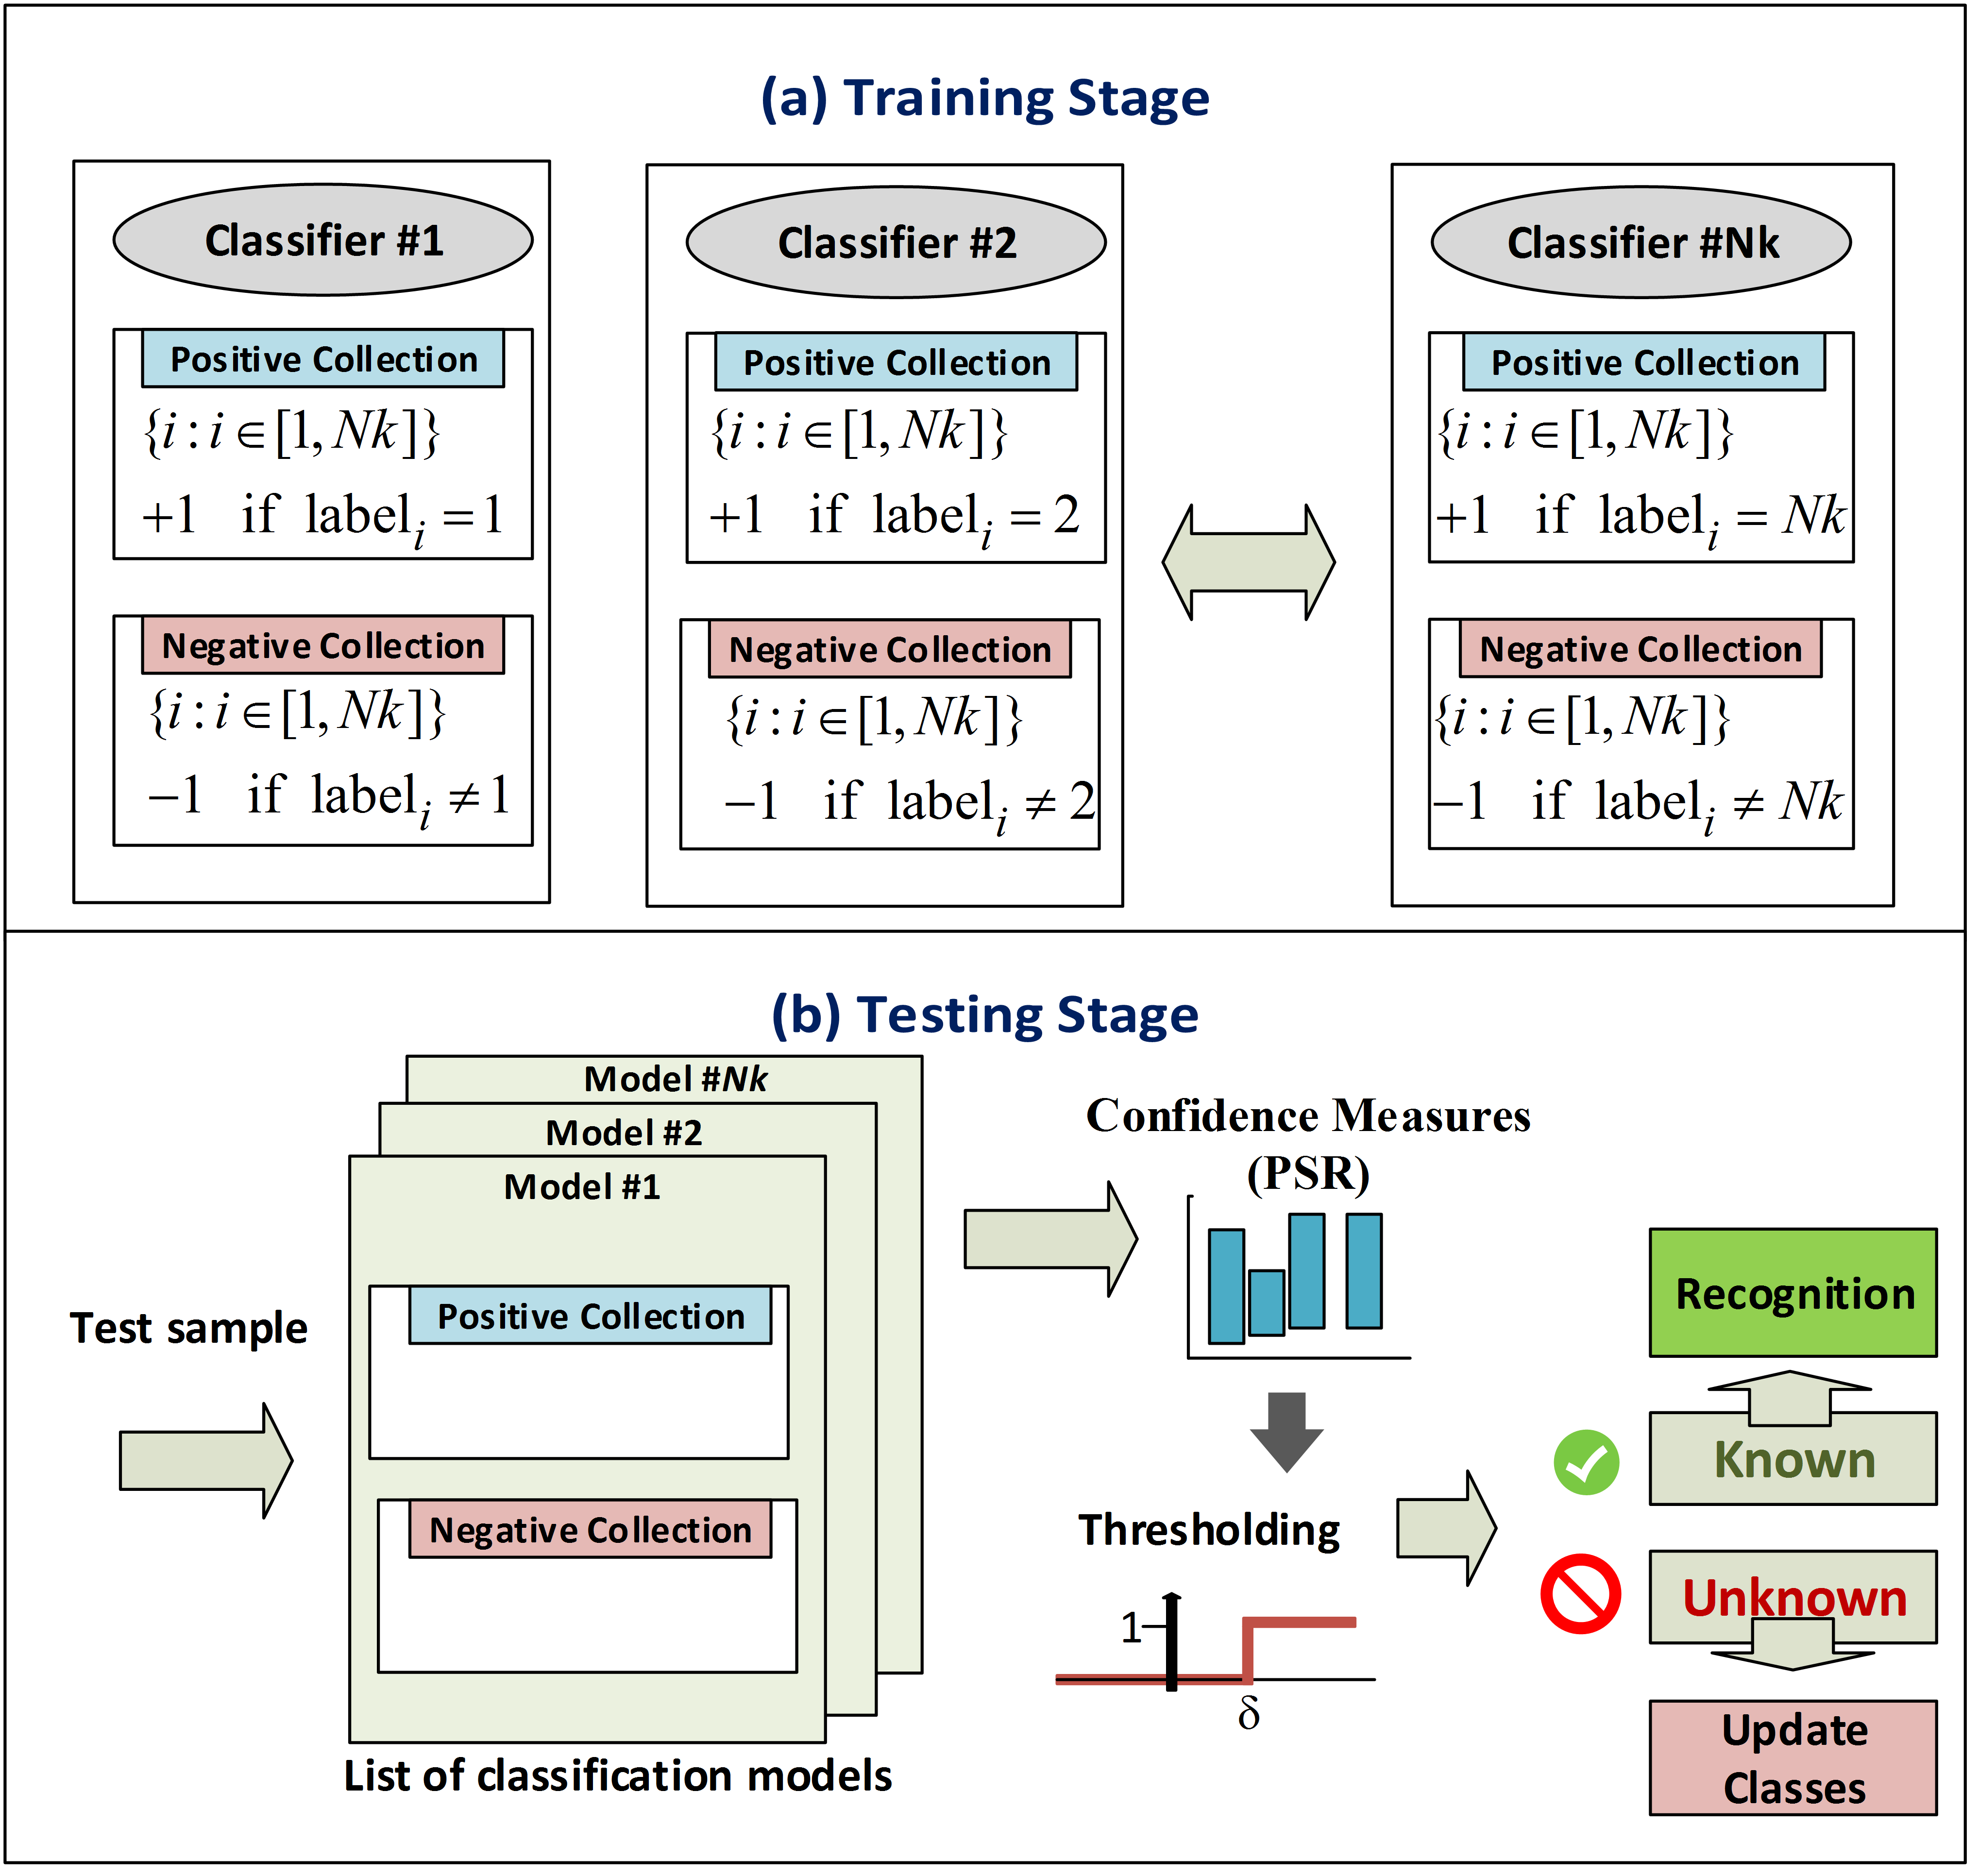
\includegraphics[width=0.45\textwidth]{img/architecture.png}
	\caption{The system architecture of the proposed method. At training, features are obtained to train different classifiers and produce models. At testing, the new samples are compared to all saved models. If the confidence measure exceeds a pre-determined threshold, it is considered a known class; otherwise, it is considered unknown.}
	\label{fig:fig2}
\end{figure}
Let us arrange posterior probability values $ P_{j} $ , where  $ j=1,...,Nk $  in descending order, where $ Nk $  is the number of classifiers, $ P_{1} $   is the largest value, and $ P_{Nk} $  is the smallest value. The PSR is then:
\begin{equation}
PSR = \left| {{P_1} - \frac{{{P_2} - {P_{Nk}}}}{{\sqrt {\frac{{\sum\nolimits_{j = 2}^{Nk} {{{({P_j} - \bar P)}^2}} }}{{Nk - 1}}} }}} \right|
\label{eq22}
\end{equation}
where $ \bar P $  is the average and $ \left|.\right| $  represents the absolute value here. When the system receives a new sample $ \hat x $ , the SVM classifiers compute posterior probability 
$P({Y_j}|\hat x)$  as in eq (\ref{eq21}). In the traditional way, they assign the new sample to a certain class $ Y_{j} $  that has an index associated with the largest probability value, but the probability estimation of unknown classes $ P({Y_{unknown}}|\hat x)$   is not possible, and $argmax$ of the probability estimation does not provide a sufficient scale when novel class data are far from any training data. The PSR is used here to make the rejection decision. If the PSR is larger than a certain threshold, the sample is rejected and labeled as an unknown class. Otherwise, the sample is assigned to the class that has the maximum posterior probability:
\begin{equation}
\hat y = \begin{cases} 
\text{$\underset{i}{\mathrm{argmax}} P({Y_i}|\hat x)$}     &    
\resizebox{0.16\hsize}{!}{$\text{if PSR  $\leq \delta$}$}  \\
\text{Unknown}     &   
\resizebox{0.16\hsize}{!}{$\text{if PSR > $\delta$}$}  
\end{cases} 
\resizebox{0.24\hsize}{!}{$\text{  }\forall i \in (1,...,Nk)$}
\label{eq23}
\end{equation}

The PSR characterizes the distribution of posterior probability values. It helps to determine the threshold for rejecting or accepting a particular class. A small PSR score gives credibility to the classifier. A high score means that the posterior probabilities are randomly distributed, which leads to a questionable classification decision, and the tested signal will be rejected. To visualize the effect of the PSR, Fig. \ref{fig:fig3} shows the histogram of PSR and posterior probabilities. It is clear that the use of the PSR is much more reliable for distinguishing new classes from predefined classes.
\begin{figure}[t!]
	\centering
	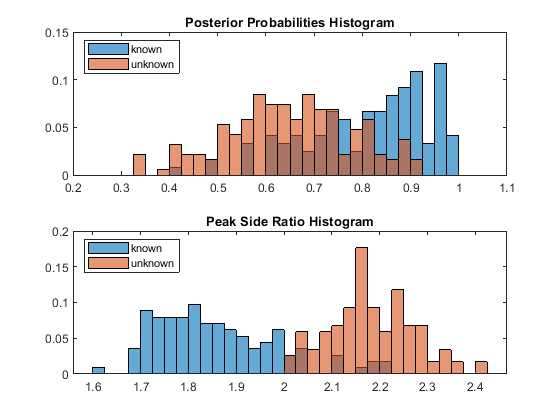
\includegraphics[width=0.5\textwidth]{img/histogram.png}
	\caption{Histograms showing the distribution of the matching rates of hypothetical testing data. The blue ones represent data from target classes, i.e., classes that are known during the training stage. The other ones represent data from the remaining classes, i.e., classes not seen during training.  }
	\label{fig:fig3}
\end{figure}
\begin{figure}[t!]
	\centering
	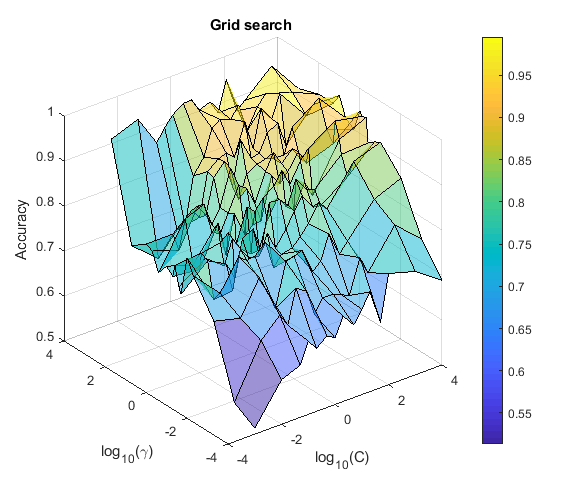
\includegraphics[width=0.45\textwidth]{img/grid.png}
	\caption{Grid search of combinations of SVM hyper-parameter values using 5-fold cross-validation to find optimum values.}
	\label{fig:fig4}
\end{figure} 


\Figure[t!]
(topskip=0pt, botskip=0pt, midskip=0pt){img/differentSYS.png}
{Different audio identification problem formulation. (a) Closed-set problem: audio samples in training and testing stages are from the same classes. (b) Open-set detection problem, audio samples in the testing stage, including new classes. (c) Open-set classification problem, where a portion of training data is used for validation.\label{fig:fig5}}


\subsection{THRESHOLDING CRITERIA}
In order to get an optimum classifier, we have to tune the decision threshold. We select $ 10\% $ of the audio samples from all classes for validation, i.e., for tuning parameters based on a grid search. The remaining data are used later for the classification experiments. The optimal threshold is determined over different threshold values in the range $\delta  \in [1,4]$, with a resolution of
$\Delta \delta  = 0.01$ . The F1-measure is computed for each threshold value. To improve the  robustness, we use five-fold stratified cross-validation, and the F1-measure values are computed as a mean ensemble. We found that the threshold $ \delta  = 2.1 $ leads to the best performance. This threshold is then considered constant throughout our experiments.

\subsection{SETUP PROTOCOLS}
The features of the validation set are used to tune the SVM training parameters. A wide range of  $ c $ and $ \gamma $ values were tested, resulting in a total of 225 pairs of ( $ c,\gamma $ ) in each fold. The 15 different values of   $c$  were 0.001, 0.01, 0.05, 0.1, 0.2, 0.5, 1, 2, 5, 10, 20, 50, 100, 1000, 10000 and the 15 different values of $ \gamma $  were 0.0001, 0.001, 0.01, 0.1, 0.2, 0.4, 0.5, 0.8, 1, 2, 5, 10, 20, 100 and 1000. Using 5-fold cross-validation and the toolbox in \cite{37}, we plotted the grid search surface, as shown in Fig.\ref{fig:fig4}. We found that the optimum hyper-parameters that give the best prediction score were  $c=100$ and $ \gamma=20 $.

For the closed-set scenario, the audio dataset is split into training and testing datasets. We use 5-folding cross-validations. In other words, from the data unused by the validation step, $20\%$ of the unused data are used for testing, and $80\%$ of the unused data are used as the training dataset to model the classifiers. The classifiers are multi-class SVM with the one-vs-all approach, where each class of events models its classifier separately. In the testing stage, a classifier fusion step is used to merge the results of multiple classifiers. The final predicted class is the one that has the maximum vote. The audio classification is performed at both frame-level and event-level. In general, event-based performance is expected to be better than frame-based performance, because the detected event class is obtained as the most frequent frame-based class detected over that whole event (statistical mode), which removes some local errors.\\
While multi-class classification for the closed set system is evaluated by tracking the correct and incorrect classification, the open set classification evaluation must keep track of incorrect multi-class classification over known categories and errors between unknown and known categories. Therefore, two types of open set experiments are conducted: reduced open-set recognition, which computes errors between known and unknown categories, and multi-class open-set recognition, which evaluates the whole system. This will be further explained in the next section.



\section{RESULTS AND DISCUSSION} \label{sec:VIII}
This section evaluates the efficiency of our proposed architectures. We conducted our experiments as shown in Fig. 5 on a closed-set scenario and an open-set scenario. We follow a cross-validation testing procedure to verify reliability in the reported results across several trials. The experiments are conducted five times. During the experiments, our procedure randomly sorted classes to be the target, known, and unknown classes, producing a gradual transition from closed-set to increasingly open-set configurations. We report the efficiency of the system for both segment-based and event-based metrics, using standard evaluation setups provided in \cite{3}. The systems are evaluated for the following types of errors:
\begin{itemize}	
	\item \emph Misclassification: Test samples misclassified with a wrong label, belonging to one of the predefined classes;
	\item \emph False unknown: Test samples rejected as unknown, but in reality, belonging to one of the predefined classes;  
	\item \emph False known: Test samples truly unknown, but assigned to one of the predefined classes.
\end{itemize}
The first task is to examine the classifiers' accuracy in closed-set recognition, where only the first type of error is possible. This task is important because it explains how well an algorithm learns the training data. Then, for open-set recognition, experiments are conducted on two different open set scenarios:  
\begin{enumerate}
	\item -	Reduced open-set recognition examines the classifiers' ability to distinguish unknown from known targets, as described in \cite{38}. For a signal labeled by the classifier as known, it does not show if it will be further correctly assigned to one of the known classes. The first type of error is not possible in this scenario.
	\item -	Multi-class open-set recognition described by Scheirer et al. \cite{2}, where a system not only rejects a target that is not seen in the training stage, but it also labels the class that a target belongs to within the known classes. In this scenario, the three types of errors are possible.
\end{enumerate}	
In order to assess the accuracy and effectiveness of our proposed method, it was compared with the following methods known in the prior art for open set recognition:
\begin{itemize}	
	\item \emph LP-SVM classifier \cite{36}: SVM classifier with a linear kernel and the posterior probabilities calibrated using Platt scaling.
	\item \emph RBF-SVM classifier \cite{19}: One-vs-all multi-class SVM classifier with Radial Basis Function (RBF) kernel, and posterior probabilities calibrated using Platt scaling.
	\item \emph 1-vs-set machine \cite{2}: a linear classifier with a one-vs-all approach. It optimizes the recognition of empirical and open space risk. We used the new version of the C code implementation provided on the website \cite{39}.
\end{itemize}

\subsection{CLOSED-SET RECOGNITION }
When $ Y_{k}=Y_{u} $,  the number of unknown acoustic classes is 0, which is a full closed-set. The training/test protocol is 5-fold cross-validation. The model of each class is trained on four sets of the class, and the model is tested using the remaining  $ 5^{th} $ fold. Since the purpose of the closed set recognition experiment is to validate the ability of our proposed algorithm to discriminate among known classes, we did not conduct comparisons with other algorithms in this part. Comparisons with other algorithms are made for open set recognition experiments in the next sub-sections.  
\begin{table}
	\caption{Overall Accuracy and F1 metric for Closed-Set Recognition}
	\centering
	\setlength{\tabcolsep}{6pt}
	\begin{tabular}{|c|c|c|c|c}		
		\cline{1-4}
		\multicolumn{2}{|c|}{\textbf{Measurement}}                             & \textbf{Frame-based} & \textbf{Event-based} &  \\ \cline{1-4}
		\multicolumn{2}{|c|}{\textbf{Accuracy}}                                & \textbf{0.891}       & \textbf{0.892}       &  \\ \cline{1-4}
		\multicolumn{1}{|c|}{\multirow{2}{*}{\textbf{F1 measure}}} & Micro Avg & 0.889                & 0.884                &  \\ \cline{2-4}
		\multicolumn{1}{|c|}{}                                     & Macro Avg & 0.853                & 0.881                &  \\ \cline{1-4}
		\multicolumn{1}{|c|}{\multirow{2}{*}{\textbf{precision}}}  & Micro Avg & 0.886                & 0.883                &  \\ \cline{2-4}
		\multicolumn{1}{|c|}{}                                     & Macro Avg & 0.861                & 0.910                &  \\ \cline{1-4}
		\multirow{2}{*}{\textbf{recall}}                           & Micro Avg & 0.887                & 0.882                &  \\ \cline{2-4}
		& Macro Avg & 0.840                & 0.884                &  \\ \cline{1-4}
	\end{tabular}
	\label{tab:table2}
\end{table}
Table \ref{tab:table2} shows the overall accuracy and F1 metrics, computed with macro-averages and micro-averages. As can be seen, there are  $ 11 \% $ mis-classifications due to the similarities among some classes. In general, the classification performance using both event-based and frame-based metrics shows that the proposed algorithm is a reliable classifier..\\
For both frame-based and event-based metrics, the confusion matrices are displayed in Fig.  \ref{fig:fig6} and fig. \ref{fig:fig7}, respectively. The matrix rows and columns refer to the ground truth and predicted labels, respectively. The matrix is normalized row-wise, as mentioned earlier. This makes all classes be considered as equal size, and the dataset becomes class-balanced. In the confusion matrix, the elements in the diagonal are correctly classified, while the elements out of the diagonal are misclassified. 
\begin{figure}[hbt!]
	\centering
	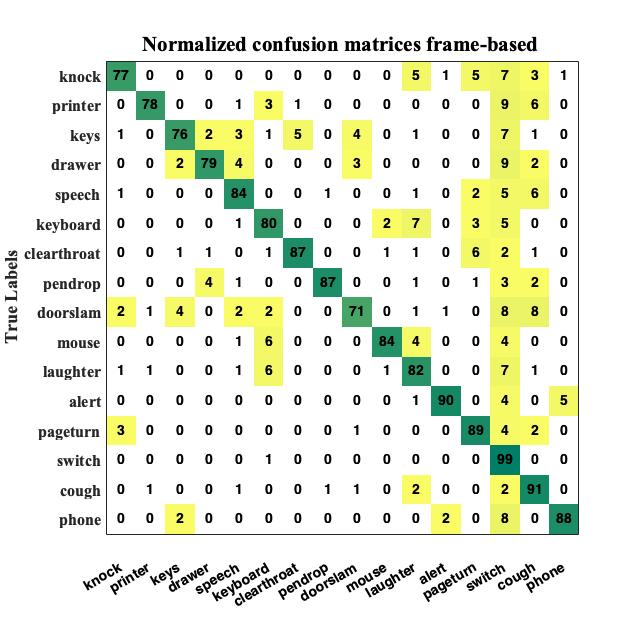
\includegraphics[width=0.5\textwidth]{img/cm_frame.png}
	\caption{Normalized confusion matrix for frame-based closed set recognition. Sixteen classes are tested in 5-fold cross-validation. Some classes have very close similarities leading to some misclassifications, such as "putting keys on the table" and "typing on keyboard", or "cough" and "speech".}
	\label{fig:fig6}
\end{figure}
\begin{figure}[hbt!]
	\centering
	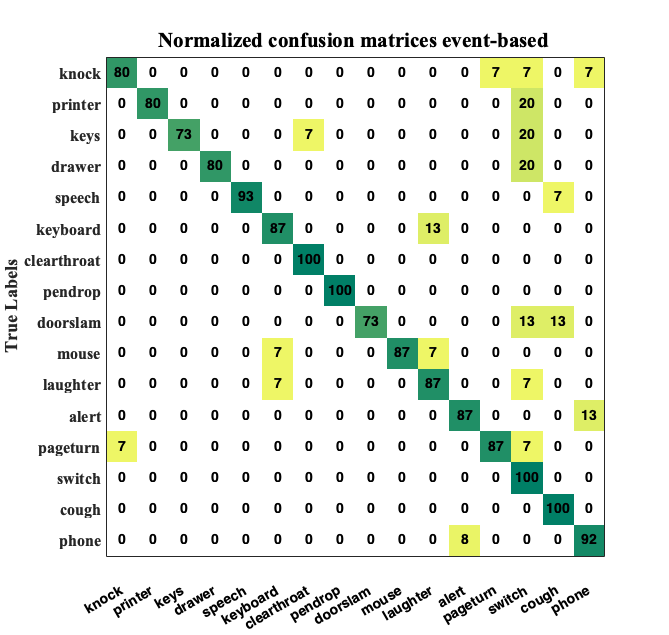
\includegraphics[width=0.5\textwidth]{img/cm_event.png}
	\caption{Normalized confusion matrix for event-based closed set recognition. Sixteen classes are tested in 5-fold cross validation. Some events have many similar frames; thus, they are misclassified, such as phone and alert, or printer and switch.}
	\label{fig:fig7}
\end{figure}
As can be seen, most of the signals are correctly classified. However, there are some cases where the system fails to distinguish classes due to strong correlation between them. It can be noticed in both figures that among the 16 classes, 'door slam' was the most difficult sound class to identify. It can be seen that it got misclassified with other classes that have a short duration, such as 'switch' and 'keys.' The macro-averaged F1-scores for the experiments of Fig.\ref{fig:fig6} and fig.\ref{fig:fig7} are respectively 0.854  and 0.892, while the micro-averaged F1-scores are 0.844 and 0.876, respectively. These scores show the expected overall better performance of event-based metrics. The closed-set results of this sub-section will be used as a baseline comparison for the open-set results of the next sub-sections, where a comparison is also made with prior art methods.

\subsection{REDUCED OPEN SET RECOGNITION}
The reduced open set performance explains how an algorithm distinguishes known from unknown data. The simulation of this scenario is done by selecting a portion of the available 
classes and considering them as known in the training and testing stages. This experiment is designed only for rejecting or accepting a new sample. It makes a decision as to whether or not a new sample belongs to the defined groups (known classes), but it does not reveal whether the correct class was assigned within the groups. Such information is considered to be expressed by closed set performance. The F1-precision and recall measures are computed, and the experiments are conducted with different numbers of target, known, and unknown classes. Table 3 shows some selected trials and our proposed algorithm's responses.The table reveals the results of the macro-average and the micro-average metrics. As described in (\ref{eq12})-(\ref{eq13}), a macro-average treats all classes equally since it computes each class independently and then takes the average of them. A micro-average combines the contribution of all classes to compute their average. Since we have more examples for some classes than others, the micro-average is preferable here.\\
 
\begin{table}
	\caption{Examples of openness as a function of number of target classes  $Y_{t}$, known classes $Y_{k}$ and unknown classes  $Y_{u}$, with corresponding F1 and AEER performance measures.}
	\centering
	\setlength{\tabcolsep}{6pt}
	\begin{tabular}{|p{10pt}|p{10pt}|p{10pt}|p{30pt}|p{45pt}|p{20pt}|p{20pt}|}
		\hline
		\textbf{$Y_{t}$}    & \textbf{$Y_{k}$}    & \textbf{$Y_{u}$}    & \textbf{Openness}                & \textbf{}                           & \textbf{F1}                   & \textbf{AEER}                 \\ \hline
		&                     &                     &                                  & \cellcolor[HTML]{C0C0C0}Frame-Based & \cellcolor[HTML]{C0C0C0}0.693 & \cellcolor[HTML]{C0C0C0}0.254 \\
		\multirow{-2}{*}{5} & \multirow{-2}{*}{6} & \multirow{-2}{*}{9} & \multirow{-2}{*}{\textbf{0.310}} & Event-Based                         & 0.697                         & 0.215                         \\
		&                     &                     &                                  & \cellcolor[HTML]{C0C0C0}Frame-Based & \cellcolor[HTML]{C0C0C0}0.705 & \cellcolor[HTML]{C0C0C0}0.253 \\
		\multirow{-2}{*}{4} & \multirow{-2}{*}{6} & \multirow{-2}{*}{4} & \multirow{-2}{*}{\textbf{0.293}} & Event-Based                         & 0.760                         & 0.146                         \\
		&                     &                     &                                  & \cellcolor[HTML]{C0C0C0}Frame-Based & \cellcolor[HTML]{C0C0C0}0.735 & \cellcolor[HTML]{C0C0C0}0.219 \\
		\multirow{-2}{*}{6} & \multirow{-2}{*}{6} & \multirow{-2}{*}{4} & \multirow{-2}{*}{\textbf{0.134}} & Event-Based                         & 0.788                         & 0.224                         \\
		&                     &                     &                                  & \cellcolor[HTML]{C0C0C0}Frame-Based & \cellcolor[HTML]{C0C0C0}0.560 & \cellcolor[HTML]{C0C0C0}0.360 \\
		\multirow{-2}{*}{3} & \multirow{-2}{*}{6} & \multirow{-2}{*}{9} & \multirow{-2}{*}{\textbf{0.466}} & Event-Based                         & 0.618                         & 0.210                         \\ \hline
	\end{tabular}
	\label{tab:table3}
\end{table}
\begin{figure}[t!]
	\centering
	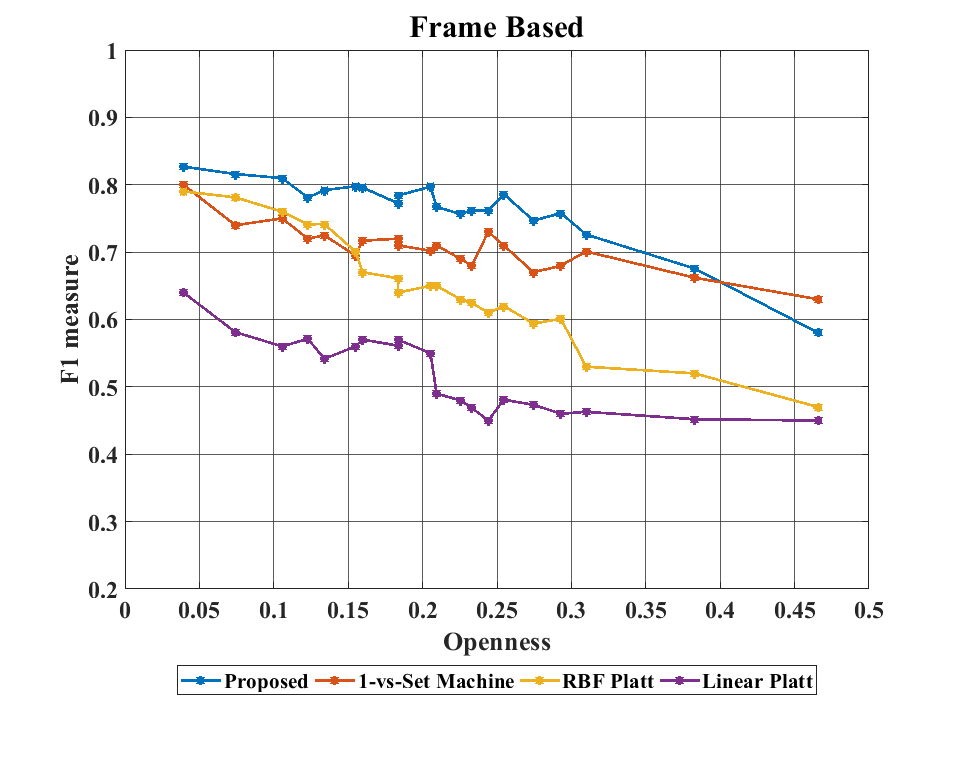
\includegraphics[width=0.5\textwidth]{img/reduced_frame.png}
	\caption{Reduced open-set recognition results as a function of openness, increasing from left to right. Results computed under frame-based metrics.}
	\label{fig:fig8}
\end{figure}

The results of the experiments evaluating reduced open set recognition for the proposed method, as well as other prior art methods, are summarized and discussed in the following. Using frame-based metrics, the results of the detection experiment for the different systems considered are shown in Fig. 8. Rejection by thresholding with linear kernel and Platt probabilities produced the worst performance. A likely explanation for this is that the linear kernel Platt classifier made the calibration model weak for unknown classes, so they were falling in between separated hyperplanes.\\

\begin{figure}[t!]
	\centering
	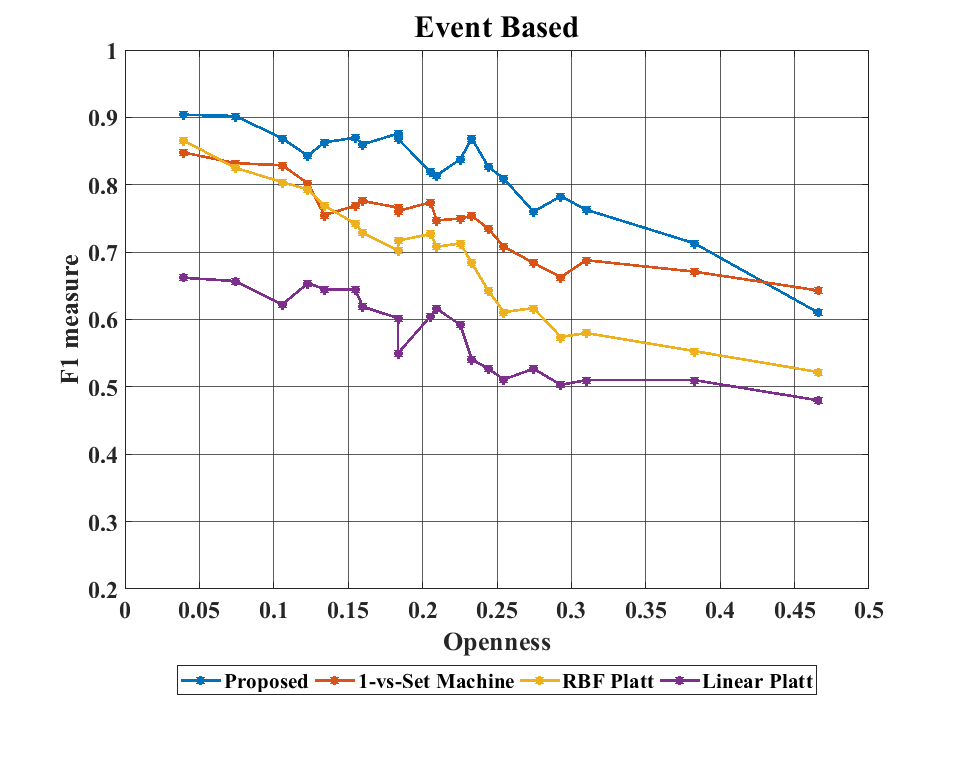
\includegraphics[width=0.5\textwidth]{img/reduced_event.png}
	\caption{F1-measure for reduced open-set recognition results as a function of openness, growing from left to right. Computed with event-based metrics.}
	\label{fig:fig9}
\end{figure}
In the same way, the reduced open-set recognition results for event-based metrics are reported in Fig. \ref{fig:fig9}. As to be expected, when more classes are available during training (less openness), the classifiers are again more accurate. We note that the performance of event-based metrics is better than the performance of frame-based metrics in Fig. \ref{fig:fig8}, for all classifiers. As the openness increases, the performance of RBF kernel Platt drops quickly, and once again, the 1-vs-set machine maintained a good performance for very open scenarios. But overall, for a wide range of openness values our proposed method again produced better results compared to other classifiers.


\subsection{MULTI-CLASS OPEN SET RECOGNITION}
In the previous subsection, the results showed the ability of our proposed method to identify and reject unknown classes and its ability to accept the known classes without labeling them. The performance of the classifiers in this subsection is evaluated for multi-class open set recognition. For multi-class recognition, we conduct these experiments on algorithms that have a rejection option. The experiments are performed by selecting six classes for training. The remaining ten classes are used as unknown data. 
\begin{figure}[t!]
	\centering
	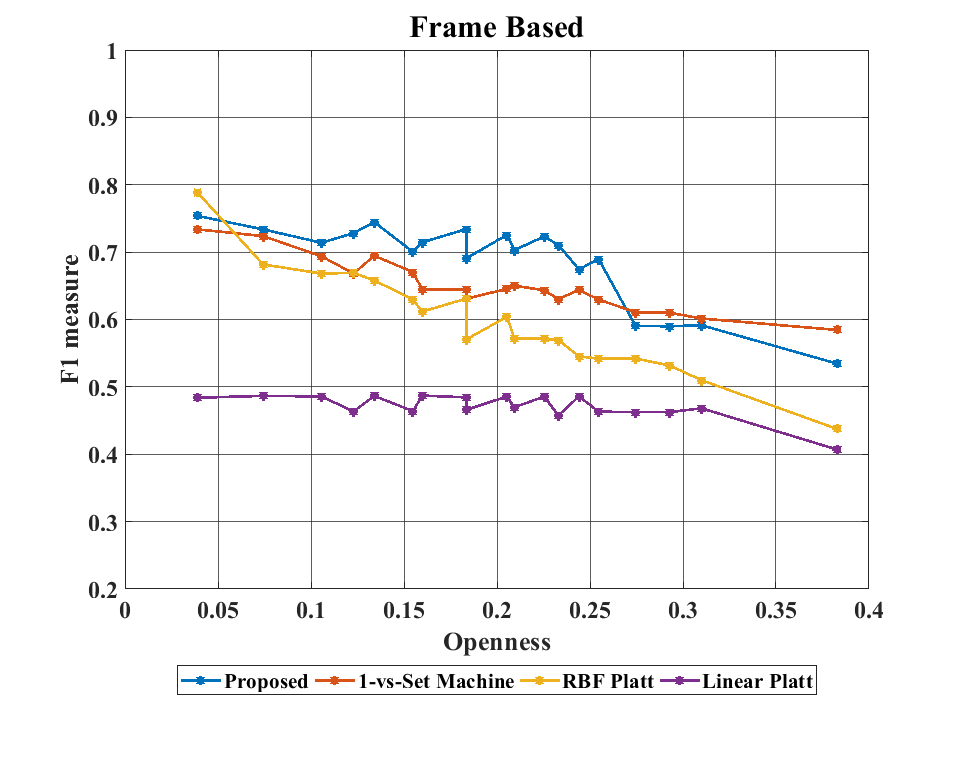
\includegraphics[width=0.5\textwidth]{img/multi_frame.png}
	\caption{F1-measure for multi-class open set recognition as a function of openness, growing from left to right. Computed with frame-based metrics.}
	\label{fig:fig10}
\end{figure}
To generate different amounts of openness, each trial selects from 1 to 10 classes of the available unknown classes, and from 2 to 6 classes to be considered as target classes. All the algorithms are executed using the same data, with the exact same negative and positive examples to sustain a fair comparison. During the testing, we consider rejected samples as either true if from an unknown class, or false if from a known class. Furthermore, the algorithms assign accepted samples to one of the known classes. The class with the maximum score, probability or votes is the predicted class. Any algorithm that does not produce a good rejection will have very poor precision as the simulation setup becomes more open, because if they miss accepting or rejecting a sample at the threshold stage, it will appear as misclassified in the metrics used.\\
\begin{figure}[t!]
	\centering
	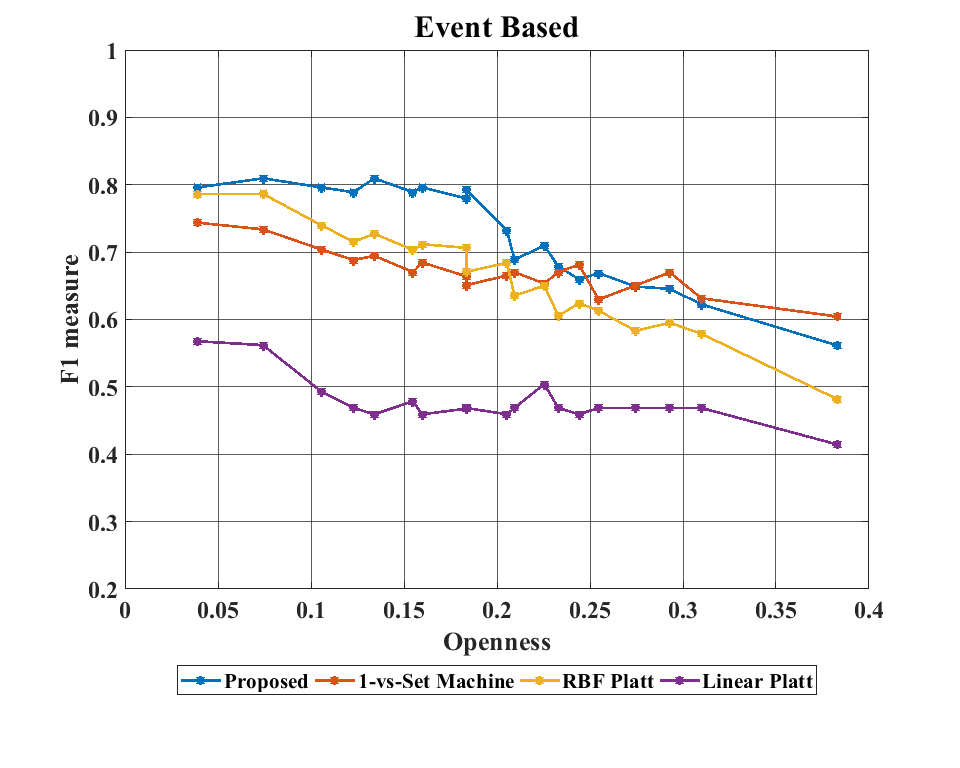
\includegraphics[width=0.5\textwidth]{img/multi_event.png}
	\caption{F1-measure for multi-class open set recognition as a function of openness, growing from left to right. Computed with event-based metrics.}
	\label{fig:fig11}
\end{figure}
For frame-based metrics, we see from Fig. \ref{fig:fig10} that our proposed method provides either the best performance or near-best performance over a wide range of openness values, for the task of separating known classes from unknown classes and distinguishing among known classes. On the other hand, the linear kernel Platt classifier is again the weakest method for this experiment. The decrease of performance as the openness of the dataset increases is again very clear for most methods.  
 
Fig. \ref{fig:fig11} shows the performance of the same simulation setups but with event-based metrics. We note that the performance of event-based metrics is again better than the performance for frame-based metrics in Fig. \ref{fig:fig10}, for all classifiers. Again our proposed method has either the best performance or near the best performance over a wide range of openness values. 
 
\section{Conclusion} \label{sec:IX}
In this work, we investigated the use of a supervised classification strategy for sound event detection and identification in an open-set scenario. Extensive experiments
were conducted using sound features proposed in the literature for closed-set audio identification. For challenging open-set scenarios, experiments using SVM classifiers were performed for recognizing known versus unknown audio events, using a threshold and a rejection function. The rejection function proposed in this paper for audio classification is a confidence measurement called the peak side ratio (PSR). It computes the distribution of posterior probabilities for all classifier outputs, to determine whether a particular measured event belongs to a certain group of known events or not. The experiments in the paper were performed on data from the DCASE 2013 challenge. Compared to previous work, our proposed method delivered the best or nearly the best performance over a wide range of openness values. However, for very large openness values, our proposed method was outperformed by the 1-vs-set machine method. \\
Overall, we demonstrated that our proposed method is promising for open set audio classification. Future work should include designing a system giving improved performance when the number of known classes is minimal.

 
\begin{thebibliography}{00}

\bibitem{1} C. Geng, S. Huang, and S. Chen, "Recent Advances in Open Set Recognition: A Survey," \textit{ArXiv181108581 Cs Sta}t, Jul. 2019, Accessed: Nov. 20, 2019. [Online]. Available: http://arxiv.org/abs/1811.08581.

\bibitem{2} W. J. Scheirer, A. D. R. Rocha, A. Sapkota, and T. E. Boult, "Toward Open Set Recognition," \textit{IEEE Trans. Pattern Anal. Mach. Intell}., vol. 35, no. 7, pp. $1757$ \textendash $1772$, Jul. 2013, doi: 10.1109/TPAMI.2012.256.

\bibitem{3} W. J. Scheirer, L. P. Jain, and T. E. Boult, "Probability Models for Open Set Recognition," \textit{IEEE Trans. Pattern Anal. Mach. Intell}., vol. 36, no. 11, pp. 2317 \textendash 2324, Nov. 2014, doi: 10.1109/TPAMI.2014.2321392

\bibitem{4} A. Mesaros, T. Heittola, and T. Virtanen, "TUT database for acoustic scene classification and sound event detection," \textit{in Signal Processing Conference (EUSIPCO)}, 2016 24th European, 2016, pp. 1128\textendash 1132. 

\bibitem{5} Fayin Li and H. Wechsler, "Open set face recognition using transduction," \textit{IEEE Trans. Pattern Anal. Mach. Intell}., vol. 27, no. 11, pp. 1686\textendash 1697, Nov. 2005, doi: 10.1109/TPAMI.2005.224.

\bibitem{6} L. M. Mazaira-Fernandez, A. Alvarez-Marquina, and P. Gomez-Vilda, "Improving speaker recognition by biometric voice deconstruction," \textit{Front. Bioeng. Biotechnol}., vol. 3, p. 126, 2015.

\bibitem{7} G. Muhammad, Y. A. Alotaibi, M. Alsulaiman, and M. N. Huda, "Environment Recognition Using Selected MPEG-7 Audio Features and Mel-Frequency Cepstral Coefficients,"\textit{ in 2010 Fifth International Conference on Digital Telecommunications (ICDT)}, Jun. 2010, pp. 11\textendash16, doi: 10.1109/ICDT.2010.10.

\bibitem{8} Y. Yang, F. Nie, D. Xu, J. Luo, Y. Zhuang, and Y. Pan, "A Multimedia Retrieval Framework Based on Semi-Supervised Ranking and Relevance Feedback," \textit{IEEE Trans. Pattern Anal. Mach. Intell.}, vol. 34, no. 4, pp. 723\textendash742, Apr. 2012, doi: 10.1109/TPAMI.2011.170.

\bibitem{9}	Y. Yang, F. Nie, D. Xu, J. Luo, Y. Zhuang, and Y. Pan, "A Multimedia Retrieval Framework Based on Semi-Supervised Ranking and Relevance Feedback," \textit{IEEE Trans. Pattern Anal. Mach. Intell}., vol. 34, no. 4, pp. 723\textendash742, Apr. 2012, doi: 10.1109/TPAMI.2011.170.
\bibitem{10}	H. Jleed and M. Bouchard, "Acoustic environment classification using discrete hartley transform features," in \textit{2017 IEEE 30th Canadian Conference on Electrical and Computer Engineering (CCECE)}, Apr. 2017, pp. 1\textendash4, doi: 10.1109/CCECE.2017.7946646.
\bibitem{11}	F.-R. Stoter, A. Liutkus, and N. Ito, "The 2018 Signal Separation Evaluation Campaign," \textit{ArXiv180406267 Cs Eess}, Apr. 2018, Accessed: Sep. 19, 2019. [Online]. Available: http://arxiv.org/abs/1804.06267.
\bibitem{12}	J. Barker, E. Vincent, N. Ma, H. Christensen, and P. Green, "The PASCAL CHiME speech separation and recognition challenge," \textit{Comput. Speech Lang}., vol. 27, no. 3, pp. 621\textendash 633, 2013.
\bibitem{13}	J. S. Downie, "The Music Information Retrieval Evaluation eXchange (MIREX)," \textit{Lib Mag}., vol. 12, no. 12, Dec. 2006, doi: 10.1045/december2006-downie.
\bibitem{14}	K. Lopatka, J. Kotus, and A. Czyzewski, "Evaluation of Sound Event Detection, Classification and Localization in the Presence of Background Noise for Acoustic Surveillance of Hazardous Situations," in \textit{Multimedia Communications, Services and Security}, A. Dziech and A. Czyżewski, Eds. Springer International Publishing, Cham, Switzerland, 2014, pp. 96\textendash110.
\bibitem{15}	A. R. Hilal, A. Sayedelahl, A. Tabibiazar, M. S. Kamel, and O. A. Basir, "A distributed sensor management for large-scale IoT indoor acoustic surveillance," \textit{Future Gener. Comput. Syst}., vol. 86, no. Complete, pp. 1170\textendash1184, 2018, doi: 10.1016/j.future.2018.01.020.
\bibitem{16}	D. Battaglino, L. Lepauloux, and N. Evans, "The open-set problem in acoustic scene classification," in \textit{2016 IEEE International Workshop on Acoustic Signal Enhancement (IWAENC)}, Sep. 2016, pp. 1\textendash5, doi: 10.1109/IWAENC.2016.7602939.
\bibitem{17}	S. Krstulovic, "Audio Event Recognition in the Smart Home," in \textit{Computational Analysis of Sound Scenes and Events}, T. Virtanen, M. D. Plumbley, and D. Ellis, Eds. Cham: Springer International Publishing, 2018, pp. 335\textendash371.
\bibitem{18}	M. Crocco, M. Cristani, A. Trucco, and V. Murino, "Audio surveillance: a systematic review,"\textit{ ACM Comput. Surv. CSUR}, vol. 48, no. 4, p. 52, 2016.
\bibitem{19}	L. P. Jain, W. J. Scheirer, and T. E. Boult, "Multi-class Open Set Recognition Using Probability of Inclusion," in \textit{Computer Vision – ECCV 2014}, vol. 8691, D. Fleet, T. Pajdla, B. Schiele, and T. Tuytelaars, Eds. Cham: Springer International Publishing, 2014, pp. 393\textendash409.
\bibitem{20}	A. Bendale and T. Boult, "Towards open world recognition," in \textit{Proceedings of the IEEE Conference on Computer Vision and Pattern Recognition, 2015}, pp. 1893\textendash1902.
\bibitem{21}	A. Bendale and T. E. Boult, "Towards Open Set Deep Networks," in \textit{2016 IEEE Conference on Computer Vision and Pattern Recognition (CVPR)}, Jun. 2016, pp. 1563 \textendash 1572, doi: 10.1109/CVPR.2016.173.
\bibitem{22}	W. J. Scheirer, A. Rocha, R. J. Micheals, and T. E. Boult, "Meta-Recognition: The Theory and Practice of Recognition Score Analysis," \textit{IEEE Trans. Pattern Anal}. Mach. Intell., vol. 33, no. 8, pp. 1689\textendash1695, Aug. 2011, doi: 10.1109/TPAMI.2011.54.
\bibitem{23}	J. D. Roos and A. K. Shaw, "Probabilistic svm for open set automatic target recognition on high range resolution radar data," in \textit{Automatic Target Recognition XXVII}. International Society for Optics and Photonics, 102020B, 2017. 
\bibitem{24}	V. Tiwari, "Mfcc and its applications in speaker recognition," Int. J. Emerg. Technol., vol. 1, no. 1, pp. 19\textendash22, 2010.
\bibitem{25}	D. Stowell, D. Giannoulis, E. Benetos, M. Lagrange, and M. D. Plumbley, "Detection and classification of acoustic scenes and events," \textit{IEEE Trans. Multimed}., vol. 17, no. 10, pp. 1733 \textendash 1746, 2015.
\bibitem{26}	J. Xin and Y. Qi, Mathematical modeling and signal processing in speech and hearing sciences. Springer Science \& Business Media, Cham, Switzerland, 2014, vol. 10.
\bibitem{27}	B. McFee et al., "Librosa: audio and music signal analysis in python," in Proceedings of the 14th python in science conference, 2015, vol. 8.
\bibitem{28}	M. Slaney, "Auditory toolbox," Interval Res. Corp. Tech Rep, vol. 10, no. 1998, 1998.
\bibitem{29}	H. Jleed and S. Agaian, "Prediction of coding region in the DNA sequences," in 2011 \textit{IEEE International Conference on Systems, Man, and Cybernetics}, Oct. 2011, pp. 1128 \textendash 1133, doi: 10.1109/ICSMC.2011.6083826.
\bibitem{30}	M. Sokolova and G. Lapalme, "A systematic analysis of performance measures for classification tasks," \textit{Inf. Process. Manag}., vol. 45, no. 4, pp. 427\textendash437, Jul. 2009, doi: 10.1016/j.ipm.2009.03.002.
\bibitem{31}	Y. Yang, "An Evaluation of Statistical Approaches to Text Categorization," \textit{Inf. Retr}., vol. 1, no. 1, pp. 69\textendash90, Apr. 1999, doi: 10.1023/A:1009982220290.
\bibitem{32}	T. Giannakopoulos and A. Pikrakis, Introduction to audio analysis: a MATLAB ® approach, First edition. Kidlington, Oxford: Academic Press is an imprint of Elsevier, 2014.
\bibitem{33}	A. Temko, C. Nadeu, D. Macho, R. Malkin, C. Zieger, and M. Omologo, "Acoustic Event Detection and Classification" \textit{in Computers in the human interaction loop}. London, U.K.: Springer, 2009, pp. 61\textendash73
\bibitem{34}	A. Diment, T. Heittola, and T. Virtanen, "Sound event detection for office live and office synthetic AASP challenge," in\textit{ IEEE AASP Challenge on Detection and Classification of Acoustic Scenes and Events (WASPAA 2013 special session)}, 2013 
\bibitem{35}	F. Font, G. Roma, and X. Serra, "Freesound technical demo," in \textit{Proceedings of the 21st ACM international conference on Multimedia}, 2013, pp. 411 \textendash 412.
\bibitem{36}	J. Platt, "Probabilistic outputs for support vector machines and comparisons to regularized likelihood methods," \textit{Adv. Large Margin Classif}., vol. 10, no. 3, pp. 61\textendash74, 1999.
\bibitem{37}	C.-C. Chang and C.-J. Lin, "LIBSVM: A library for support vector machines," \textit{ACM Trans. Intell. Syst. Technol}., vol. 2, no. 3, pp. 1 \textendash 27, Apr. 2011, doi: 10.1145/1961189.1961199.
\bibitem{38}	M. D. Scherreik and B. D. Rigling, "Open set recognition for automatic target classification with rejection," \textit{IEEE Trans. Aerosp. Electron. Syst}., vol. 52, no. 2, pp. 632\textendash 642, Apr. 2016, doi: 10.1109/TAES.2015.150027.
\bibitem{39}	W. J. Scheirer, "Open Set Recognition." https://www.wjscheirer.com/projects/openset-recognition/ (accessed Dec. 23, 2019).


\end{thebibliography}

\begin{IEEEbiography}[{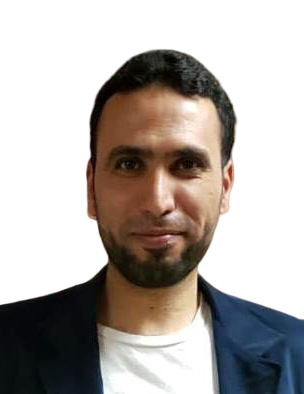
\includegraphics[width=1in,height=1.25in,clip,keepaspectratio]{img/a1.png}}]{Hitham Jleed} received a B.Sc. degree in Electronics and Computer Engineering from Sebha University, Libya, in 2004, and a M.Sc. degree in Electrical Engineering from the University of Texas at San Antonio, USA, in 2011. 

He is currently working towardsa Ph.D. degree in Electrical and Computer Engineering at the University of Ottawa, Canada. His doctoral research focuses on audio-basis surveillance applications. His research interests include applied signal processing and machine learning, with an emphasis on audio processing. He worked as a full-time lecturer at the Department of Electrical and Computer Engineering, Elmergib University, Libya, from 2011 to 2014. 
\end{IEEEbiography}

\begin{IEEEbiography}[{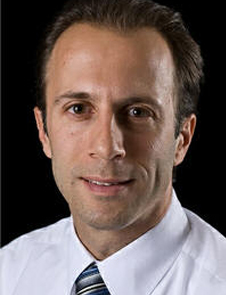
\includegraphics[width=1in,height=1.25in,clip,keepaspectratio]{img/a2.png}}]{Martin Bouchard } received the B.Ing., M.Sc.A., and Ph.D. degrees in electrical engineering from the Université de Sherbrooke, Sherbrooke, QC, Canada, in 1993, 1995, and 1997, respectively. In January 1998, he joined the School of Electrical Engineering and Computer Science, Faculty of Engineering, University of Ottawa, Ottawa, ON, Canada. In 1996, he co-founded SoftdB Inc., Quebec City, QC, which is still active today.
	
Over the years, he has conducted research activities and consulting activities with more than 20 private sector and governmental partners, supervised more than 50 graduate students and postdoctoral fellows, and authored or coauthored more than 40 journal papers and 85 conference papers. His current research interests include signal processing methods in general and machine learning, with an emphasis on speech, audio, acoustics, hearing aids, and biomedical engineering applications. He served as a member of the Speech and Language Technical Committee of the IEEE Signal Processing Society from 2009 to 2011, as an Associate Editor for the EURASIP Journal on Audio, Speech and Music Processing from 2006 to 2011, and as an Associate Editor for the IEEE TRANSACTIONS ON NEURAL NETWORKS from 2008 to 2009. He is a member of the Ordre des Ingénieurs du Québec. 
\end{IEEEbiography}

\EOD

\end{document}
